\documentclass[border=6pt]{standalone}
\usepackage[T1]{fontenc}
\usepackage[utf8]{inputenc}
\usepackage{mathptmx}
\usepackage{amsmath,amssymb,amsfonts,mathrsfs}
\usepackage[dvipsnames]{xcolor}
\usepackage{tikz}
\usetikzlibrary{calc,positioning,arrows.meta,decorations.pathreplacing,
                decorations.markings,matrix,fit,backgrounds,shapes.misc}
\renewcommand{\sl}{\mathfrak{sl}}
\newcommand{\Uq}{U_q(\sl_2)}
\newcommand{\qint}[1]{[#1]_q}
\newcommand{\Rcheck}{\check{R}}
\definecolor{accent}{RGB}{59,91,146}
\definecolor{accentsoft}{RGB}{155,180,216}
\definecolor{oddsign}{RGB}{138,40,132}
\tikzset{
  strand/.style={line width=1pt, accent!80!black},
  rbox/.style={draw=accent!70!black, fill=accentsoft!55, rounded corners=2pt,
               line width=0.8pt, minimum height=6mm},
  rdot/.style={circle, fill=accent, inner sep=1.6pt},
  knode/.style={circle, draw=accent!70!black, fill=accentsoft!45,
                line width=0.8pt, minimum size=7mm, font=\small},
  kedge/.style={accent!70!black, line width=0.9pt},
  faredge/.style={oddsign!75!black, line width=0.9pt, densely dashed},
  glabel/.style={font=\footnotesize, accent!60!black},
}
\begin{document}
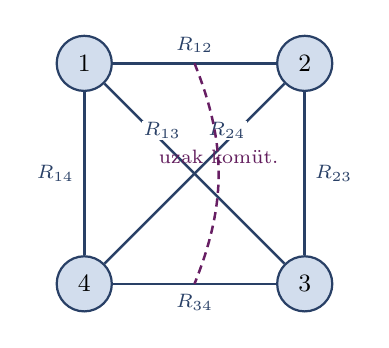
\begin{tikzpicture}[x=1.4cm,y=1.4cm]
  \node[knode] (n1) at (0,2) {1};
  \node[knode] (n2) at (2,2) {2};
  \node[knode] (n3) at (2,0) {3};
  \node[knode] (n4) at (0,0) {4};
  % 6 kenar = 6 R_{ij}
  \draw[kedge] (n1)--(n2) node[midway,above,font=\scriptsize]{$R_{12}$};
  \draw[kedge] (n2)--(n3) node[midway,right,font=\scriptsize]{$R_{23}$};
  \draw[kedge] (n3)--(n4) node[midway,below,font=\scriptsize]{$R_{34}$};
  \draw[kedge] (n1)--(n4) node[midway,left,font=\scriptsize]{$R_{14}$};
  \draw[kedge] (n1)--(n3) node[pos=0.32,above,font=\scriptsize,fill=white,inner sep=0.5pt]{$R_{13}$};
  \draw[kedge] (n2)--(n4) node[pos=0.32,above,font=\scriptsize,fill=white,inner sep=0.5pt]{$R_{24}$};
  % uzak komutativite vurgusu (12)-(34)
  \draw[faredge] ($(n1)!0.5!(n2)$) to[bend left=22] node[above,font=\scriptsize,oddsign!70!black]{uzak komüt.} ($(n3)!0.5!(n4)$);
\end{tikzpicture}
\end{document}
